% Created by tikzDevice version 0.10.1 on 2016-12-02 11:15:39
% !TEX encoding = UTF-8 Unicode
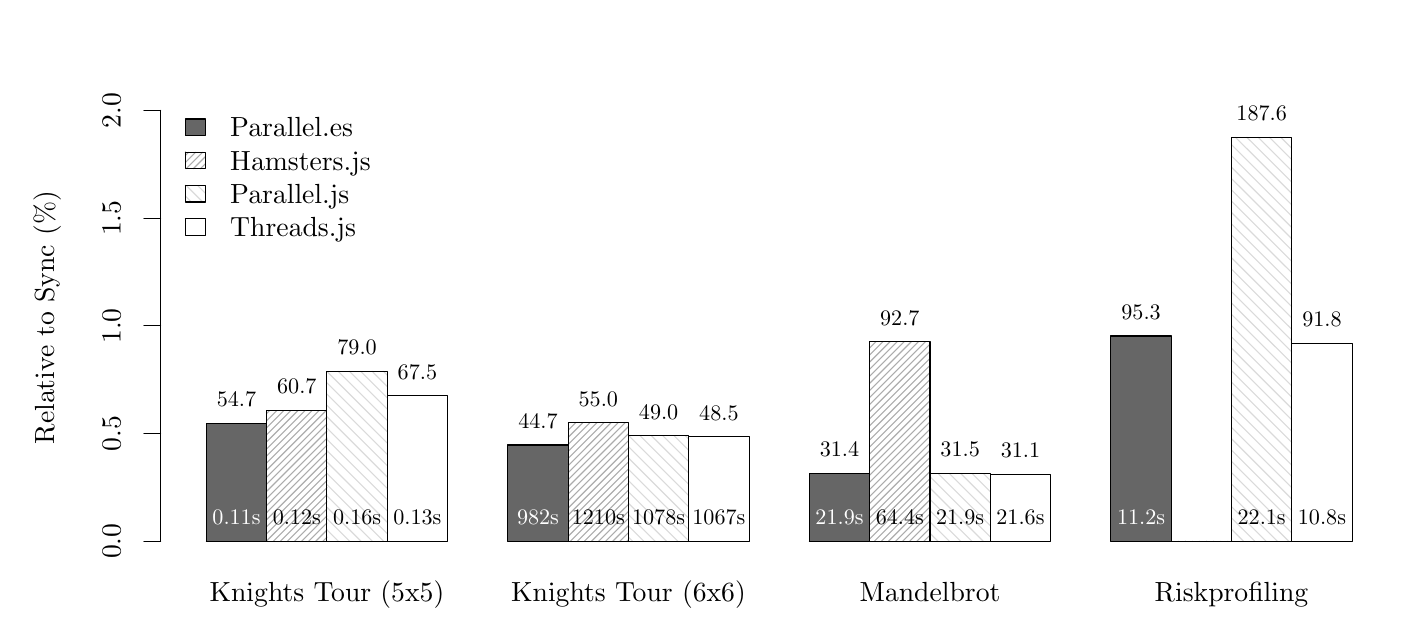
\begin{tikzpicture}[x=1pt,y=1pt]
\definecolor{fillColor}{RGB}{255,255,255}
\path[use as bounding box,fill=fillColor,fill opacity=0.00] (0,0) rectangle (495.15,209.58);
\begin{scope}
\path[clip] (  0.00,  0.00) rectangle (495.15,209.58);
\definecolor{fillColor}{gray}{0.40}

\path[fill=fillColor] ( 64.56, 24.00) --
	( 86.35, 24.00) --
	( 86.35, 66.54) --
	( 64.56, 66.54) --
	cycle;
\definecolor{drawColor}{RGB}{172,172,172}

\path[draw=drawColor,line width= 0.4pt,line join=round,line cap=round] ( 86.35, 70.14) -- ( 87.45, 71.24);

\path[draw=drawColor,line width= 0.4pt,line join=round,line cap=round] ( 86.35, 67.58) -- ( 90.01, 71.24);

\path[draw=drawColor,line width= 0.4pt,line join=round,line cap=round] ( 86.35, 65.03) -- ( 92.56, 71.24);

\path[draw=drawColor,line width= 0.4pt,line join=round,line cap=round] ( 86.35, 62.47) -- ( 95.12, 71.24);

\path[draw=drawColor,line width= 0.4pt,line join=round,line cap=round] ( 86.35, 59.92) -- ( 97.67, 71.24);

\path[draw=drawColor,line width= 0.4pt,line join=round,line cap=round] ( 86.35, 57.36) -- (100.23, 71.24);

\path[draw=drawColor,line width= 0.4pt,line join=round,line cap=round] ( 86.35, 54.81) -- (102.78, 71.24);

\path[draw=drawColor,line width= 0.4pt,line join=round,line cap=round] ( 86.35, 52.25) -- (105.34, 71.24);

\path[draw=drawColor,line width= 0.4pt,line join=round,line cap=round] ( 86.35, 49.70) -- (107.89, 71.24);

\path[draw=drawColor,line width= 0.4pt,line join=round,line cap=round] ( 86.35, 47.14) -- (108.14, 68.93);

\path[draw=drawColor,line width= 0.4pt,line join=round,line cap=round] ( 86.35, 44.59) -- (108.14, 66.38);

\path[draw=drawColor,line width= 0.4pt,line join=round,line cap=round] ( 86.35, 42.03) -- (108.14, 63.82);

\path[draw=drawColor,line width= 0.4pt,line join=round,line cap=round] ( 86.35, 39.48) -- (108.14, 61.27);

\path[draw=drawColor,line width= 0.4pt,line join=round,line cap=round] ( 86.35, 36.92) -- (108.14, 58.71);

\path[draw=drawColor,line width= 0.4pt,line join=round,line cap=round] ( 86.35, 34.36) -- (108.14, 56.16);

\path[draw=drawColor,line width= 0.4pt,line join=round,line cap=round] ( 86.35, 31.81) -- (108.14, 53.60);

\path[draw=drawColor,line width= 0.4pt,line join=round,line cap=round] ( 86.35, 29.25) -- (108.14, 51.05);

\path[draw=drawColor,line width= 0.4pt,line join=round,line cap=round] ( 86.35, 26.70) -- (108.14, 48.49);

\path[draw=drawColor,line width= 0.4pt,line join=round,line cap=round] ( 86.35, 24.14) -- (108.14, 45.94);

\path[draw=drawColor,line width= 0.4pt,line join=round,line cap=round] ( 88.76, 24.00) -- (108.14, 43.38);

\path[draw=drawColor,line width= 0.4pt,line join=round,line cap=round] ( 91.32, 24.00) -- (108.14, 40.82);

\path[draw=drawColor,line width= 0.4pt,line join=round,line cap=round] ( 93.87, 24.00) -- (108.14, 38.27);

\path[draw=drawColor,line width= 0.4pt,line join=round,line cap=round] ( 96.43, 24.00) -- (108.14, 35.71);

\path[draw=drawColor,line width= 0.4pt,line join=round,line cap=round] ( 98.98, 24.00) -- (108.14, 33.16);

\path[draw=drawColor,line width= 0.4pt,line join=round,line cap=round] (101.54, 24.00) -- (108.14, 30.60);

\path[draw=drawColor,line width= 0.4pt,line join=round,line cap=round] (104.09, 24.00) -- (108.14, 28.05);

\path[draw=drawColor,line width= 0.4pt,line join=round,line cap=round] (106.65, 24.00) -- (108.14, 25.49);
\definecolor{drawColor}{RGB}{218,218,218}

\path[draw=drawColor,line width= 0.4pt,line join=round,line cap=round] (108.18, 24.00) -- (108.14, 24.04);

\path[draw=drawColor,line width= 0.4pt,line join=round,line cap=round] (112.27, 24.00) -- (108.14, 28.13);

\path[draw=drawColor,line width= 0.4pt,line join=round,line cap=round] (116.36, 24.00) -- (108.14, 32.22);

\path[draw=drawColor,line width= 0.4pt,line join=round,line cap=round] (120.45, 24.00) -- (108.14, 36.30);

\path[draw=drawColor,line width= 0.4pt,line join=round,line cap=round] (124.53, 24.00) -- (108.14, 40.39);

\path[draw=drawColor,line width= 0.4pt,line join=round,line cap=round] (128.62, 24.00) -- (108.14, 44.48);

\path[draw=drawColor,line width= 0.4pt,line join=round,line cap=round] (129.93, 26.78) -- (108.14, 48.57);

\path[draw=drawColor,line width= 0.4pt,line join=round,line cap=round] (129.93, 30.87) -- (108.14, 52.66);

\path[draw=drawColor,line width= 0.4pt,line join=round,line cap=round] (129.93, 34.95) -- (108.14, 56.74);

\path[draw=drawColor,line width= 0.4pt,line join=round,line cap=round] (129.93, 39.04) -- (108.14, 60.83);

\path[draw=drawColor,line width= 0.4pt,line join=round,line cap=round] (129.93, 43.13) -- (108.14, 64.92);

\path[draw=drawColor,line width= 0.4pt,line join=round,line cap=round] (129.93, 47.22) -- (108.14, 69.01);

\path[draw=drawColor,line width= 0.4pt,line join=round,line cap=round] (129.93, 51.31) -- (108.14, 73.10);

\path[draw=drawColor,line width= 0.4pt,line join=round,line cap=round] (129.93, 55.39) -- (108.14, 77.19);

\path[draw=drawColor,line width= 0.4pt,line join=round,line cap=round] (129.93, 59.48) -- (108.14, 81.27);

\path[draw=drawColor,line width= 0.4pt,line join=round,line cap=round] (129.93, 63.57) -- (108.14, 85.36);

\path[draw=drawColor,line width= 0.4pt,line join=round,line cap=round] (129.93, 67.66) -- (112.15, 85.44);

\path[draw=drawColor,line width= 0.4pt,line join=round,line cap=round] (129.93, 71.75) -- (116.24, 85.44);

\path[draw=drawColor,line width= 0.4pt,line join=round,line cap=round] (129.93, 75.84) -- (120.33, 85.44);

\path[draw=drawColor,line width= 0.4pt,line join=round,line cap=round] (129.93, 79.92) -- (124.42, 85.44);

\path[draw=drawColor,line width= 0.4pt,line join=round,line cap=round] (129.93, 84.01) -- (128.51, 85.44);

\path[fill=fillColor] (173.51, 24.00) --
	(195.31, 24.00) --
	(195.31, 58.77) --
	(173.51, 58.77) --
	cycle;
\definecolor{drawColor}{RGB}{172,172,172}

\path[draw=drawColor,line width= 0.4pt,line join=round,line cap=round] (195.31, 66.66) -- (195.46, 66.82);

\path[draw=drawColor,line width= 0.4pt,line join=round,line cap=round] (195.31, 64.11) -- (198.02, 66.82);

\path[draw=drawColor,line width= 0.4pt,line join=round,line cap=round] (195.31, 61.55) -- (200.57, 66.82);

\path[draw=drawColor,line width= 0.4pt,line join=round,line cap=round] (195.31, 59.00) -- (203.13, 66.82);

\path[draw=drawColor,line width= 0.4pt,line join=round,line cap=round] (195.31, 56.44) -- (205.68, 66.82);

\path[draw=drawColor,line width= 0.4pt,line join=round,line cap=round] (195.31, 53.89) -- (208.24, 66.82);

\path[draw=drawColor,line width= 0.4pt,line join=round,line cap=round] (195.31, 51.33) -- (210.79, 66.82);

\path[draw=drawColor,line width= 0.4pt,line join=round,line cap=round] (195.31, 48.78) -- (213.35, 66.82);

\path[draw=drawColor,line width= 0.4pt,line join=round,line cap=round] (195.31, 46.22) -- (215.90, 66.82);

\path[draw=drawColor,line width= 0.4pt,line join=round,line cap=round] (195.31, 43.67) -- (217.10, 65.46);

\path[draw=drawColor,line width= 0.4pt,line join=round,line cap=round] (195.31, 41.11) -- (217.10, 62.90);

\path[draw=drawColor,line width= 0.4pt,line join=round,line cap=round] (195.31, 38.56) -- (217.10, 60.35);

\path[draw=drawColor,line width= 0.4pt,line join=round,line cap=round] (195.31, 36.00) -- (217.10, 57.79);

\path[draw=drawColor,line width= 0.4pt,line join=round,line cap=round] (195.31, 33.45) -- (217.10, 55.24);

\path[draw=drawColor,line width= 0.4pt,line join=round,line cap=round] (195.31, 30.89) -- (217.10, 52.68);

\path[draw=drawColor,line width= 0.4pt,line join=round,line cap=round] (195.31, 28.34) -- (217.10, 50.13);

\path[draw=drawColor,line width= 0.4pt,line join=round,line cap=round] (195.31, 25.78) -- (217.10, 47.57);

\path[draw=drawColor,line width= 0.4pt,line join=round,line cap=round] (196.08, 24.00) -- (217.10, 45.02);

\path[draw=drawColor,line width= 0.4pt,line join=round,line cap=round] (198.63, 24.00) -- (217.10, 42.46);

\path[draw=drawColor,line width= 0.4pt,line join=round,line cap=round] (201.19, 24.00) -- (217.10, 39.91);

\path[draw=drawColor,line width= 0.4pt,line join=round,line cap=round] (203.74, 24.00) -- (217.10, 37.35);

\path[draw=drawColor,line width= 0.4pt,line join=round,line cap=round] (206.30, 24.00) -- (217.10, 34.80);

\path[draw=drawColor,line width= 0.4pt,line join=round,line cap=round] (208.85, 24.00) -- (217.10, 32.24);

\path[draw=drawColor,line width= 0.4pt,line join=round,line cap=round] (211.41, 24.00) -- (217.10, 29.69);

\path[draw=drawColor,line width= 0.4pt,line join=round,line cap=round] (213.96, 24.00) -- (217.10, 27.13);

\path[draw=drawColor,line width= 0.4pt,line join=round,line cap=round] (216.52, 24.00) -- (217.10, 24.58);
\definecolor{drawColor}{RGB}{218,218,218}

\path[draw=drawColor,line width= 0.4pt,line join=round,line cap=round] (218.56, 24.00) -- (217.10, 25.47);

\path[draw=drawColor,line width= 0.4pt,line join=round,line cap=round] (222.65, 24.00) -- (217.10, 29.55);

\path[draw=drawColor,line width= 0.4pt,line join=round,line cap=round] (226.74, 24.00) -- (217.10, 33.64);

\path[draw=drawColor,line width= 0.4pt,line join=round,line cap=round] (230.83, 24.00) -- (217.10, 37.73);

\path[draw=drawColor,line width= 0.4pt,line join=round,line cap=round] (234.92, 24.00) -- (217.10, 41.82);

\path[draw=drawColor,line width= 0.4pt,line join=round,line cap=round] (238.89, 24.12) -- (217.10, 45.91);

\path[draw=drawColor,line width= 0.4pt,line join=round,line cap=round] (238.89, 28.21) -- (217.10, 50.00);

\path[draw=drawColor,line width= 0.4pt,line join=round,line cap=round] (238.89, 32.29) -- (217.10, 54.08);

\path[draw=drawColor,line width= 0.4pt,line join=round,line cap=round] (238.89, 36.38) -- (217.10, 58.17);

\path[draw=drawColor,line width= 0.4pt,line join=round,line cap=round] (238.89, 40.47) -- (217.21, 62.15);

\path[draw=drawColor,line width= 0.4pt,line join=round,line cap=round] (238.89, 44.56) -- (221.30, 62.15);

\path[draw=drawColor,line width= 0.4pt,line join=round,line cap=round] (238.89, 48.65) -- (225.39, 62.15);

\path[draw=drawColor,line width= 0.4pt,line join=round,line cap=round] (238.89, 52.73) -- (229.48, 62.15);

\path[draw=drawColor,line width= 0.4pt,line join=round,line cap=round] (238.89, 56.82) -- (233.56, 62.15);

\path[draw=drawColor,line width= 0.4pt,line join=round,line cap=round] (238.89, 60.91) -- (237.65, 62.15);

\path[fill=fillColor] (282.47, 24.00) --
	(304.26, 24.00) --
	(304.26, 48.47) --
	(282.47, 48.47) --
	cycle;
\definecolor{drawColor}{RGB}{172,172,172}

\path[draw=drawColor,line width= 0.4pt,line join=round,line cap=round] (304.26, 93.85) -- (306.52, 96.12);

\path[draw=drawColor,line width= 0.4pt,line join=round,line cap=round] (304.26, 91.30) -- (309.08, 96.12);

\path[draw=drawColor,line width= 0.4pt,line join=round,line cap=round] (304.26, 88.74) -- (311.63, 96.12);

\path[draw=drawColor,line width= 0.4pt,line join=round,line cap=round] (304.26, 86.19) -- (314.19, 96.12);

\path[draw=drawColor,line width= 0.4pt,line join=round,line cap=round] (304.26, 83.63) -- (316.74, 96.12);

\path[draw=drawColor,line width= 0.4pt,line join=round,line cap=round] (304.26, 81.08) -- (319.30, 96.12);

\path[draw=drawColor,line width= 0.4pt,line join=round,line cap=round] (304.26, 78.52) -- (321.85, 96.12);

\path[draw=drawColor,line width= 0.4pt,line join=round,line cap=round] (304.26, 75.97) -- (324.41, 96.12);

\path[draw=drawColor,line width= 0.4pt,line join=round,line cap=round] (304.26, 73.41) -- (326.05, 95.20);

\path[draw=drawColor,line width= 0.4pt,line join=round,line cap=round] (304.26, 70.86) -- (326.05, 92.65);

\path[draw=drawColor,line width= 0.4pt,line join=round,line cap=round] (304.26, 68.30) -- (326.05, 90.09);

\path[draw=drawColor,line width= 0.4pt,line join=round,line cap=round] (304.26, 65.75) -- (326.05, 87.54);

\path[draw=drawColor,line width= 0.4pt,line join=round,line cap=round] (304.26, 63.19) -- (326.05, 84.98);

\path[draw=drawColor,line width= 0.4pt,line join=round,line cap=round] (304.26, 60.64) -- (326.05, 82.43);

\path[draw=drawColor,line width= 0.4pt,line join=round,line cap=round] (304.26, 58.08) -- (326.05, 79.87);

\path[draw=drawColor,line width= 0.4pt,line join=round,line cap=round] (304.26, 55.53) -- (326.05, 77.32);

\path[draw=drawColor,line width= 0.4pt,line join=round,line cap=round] (304.26, 52.97) -- (326.05, 74.76);

\path[draw=drawColor,line width= 0.4pt,line join=round,line cap=round] (304.26, 50.42) -- (326.05, 72.21);

\path[draw=drawColor,line width= 0.4pt,line join=round,line cap=round] (304.26, 47.86) -- (326.05, 69.65);

\path[draw=drawColor,line width= 0.4pt,line join=round,line cap=round] (304.26, 45.31) -- (326.05, 67.10);

\path[draw=drawColor,line width= 0.4pt,line join=round,line cap=round] (304.26, 42.75) -- (326.05, 64.54);

\path[draw=drawColor,line width= 0.4pt,line join=round,line cap=round] (304.26, 40.20) -- (326.05, 61.99);

\path[draw=drawColor,line width= 0.4pt,line join=round,line cap=round] (304.26, 37.64) -- (326.05, 59.43);

\path[draw=drawColor,line width= 0.4pt,line join=round,line cap=round] (304.26, 35.09) -- (326.05, 56.88);

\path[draw=drawColor,line width= 0.4pt,line join=round,line cap=round] (304.26, 32.53) -- (326.05, 54.32);

\path[draw=drawColor,line width= 0.4pt,line join=round,line cap=round] (304.26, 29.98) -- (326.05, 51.77);

\path[draw=drawColor,line width= 0.4pt,line join=round,line cap=round] (304.26, 27.42) -- (326.05, 49.21);

\path[draw=drawColor,line width= 0.4pt,line join=round,line cap=round] (304.26, 24.87) -- (326.05, 46.66);

\path[draw=drawColor,line width= 0.4pt,line join=round,line cap=round] (305.95, 24.00) -- (326.05, 44.10);

\path[draw=drawColor,line width= 0.4pt,line join=round,line cap=round] (308.50, 24.00) -- (326.05, 41.55);

\path[draw=drawColor,line width= 0.4pt,line join=round,line cap=round] (311.06, 24.00) -- (326.05, 38.99);

\path[draw=drawColor,line width= 0.4pt,line join=round,line cap=round] (313.61, 24.00) -- (326.05, 36.44);

\path[draw=drawColor,line width= 0.4pt,line join=round,line cap=round] (316.17, 24.00) -- (326.05, 33.88);

\path[draw=drawColor,line width= 0.4pt,line join=round,line cap=round] (318.72, 24.00) -- (326.05, 31.33);

\path[draw=drawColor,line width= 0.4pt,line join=round,line cap=round] (321.28, 24.00) -- (326.05, 28.77);

\path[draw=drawColor,line width= 0.4pt,line join=round,line cap=round] (323.83, 24.00) -- (326.05, 26.22);
\definecolor{drawColor}{RGB}{218,218,218}

\path[draw=drawColor,line width= 0.4pt,line join=round,line cap=round] (328.94, 24.00) -- (326.05, 26.89);

\path[draw=drawColor,line width= 0.4pt,line join=round,line cap=round] (333.03, 24.00) -- (326.05, 30.98);

\path[draw=drawColor,line width= 0.4pt,line join=round,line cap=round] (337.12, 24.00) -- (326.05, 35.07);

\path[draw=drawColor,line width= 0.4pt,line join=round,line cap=round] (341.21, 24.00) -- (326.05, 39.16);

\path[draw=drawColor,line width= 0.4pt,line join=round,line cap=round] (345.30, 24.00) -- (326.05, 43.25);

\path[draw=drawColor,line width= 0.4pt,line join=round,line cap=round] (347.84, 25.54) -- (326.05, 47.34);

\path[draw=drawColor,line width= 0.4pt,line join=round,line cap=round] (347.84, 29.63) -- (328.98, 48.49);

\path[draw=drawColor,line width= 0.4pt,line join=round,line cap=round] (347.84, 33.72) -- (333.07, 48.49);

\path[draw=drawColor,line width= 0.4pt,line join=round,line cap=round] (347.84, 37.81) -- (337.16, 48.49);

\path[draw=drawColor,line width= 0.4pt,line join=round,line cap=round] (347.84, 41.90) -- (341.25, 48.49);

\path[draw=drawColor,line width= 0.4pt,line join=round,line cap=round] (347.84, 45.99) -- (345.34, 48.49);

\path[fill=fillColor] (391.42, 24.00) --
	(413.21, 24.00) --
	(413.21, 98.17) --
	(391.42, 98.17) --
	cycle;
\definecolor{drawColor}{RGB}{172,172,172}

\path[draw=drawColor,line width= 0.4pt,line join=round,line cap=round] (413.26, 24.00) -- (413.26, 24.00);

\path[draw=drawColor,line width= 0.4pt,line join=round,line cap=round] (415.82, 24.00) -- (415.82, 24.00);

\path[draw=drawColor,line width= 0.4pt,line join=round,line cap=round] (418.37, 24.00) -- (418.37, 24.00);

\path[draw=drawColor,line width= 0.4pt,line join=round,line cap=round] (420.93, 24.00) -- (420.93, 24.00);

\path[draw=drawColor,line width= 0.4pt,line join=round,line cap=round] (423.48, 24.00) -- (423.48, 24.00);

\path[draw=drawColor,line width= 0.4pt,line join=round,line cap=round] (426.04, 24.00) -- (426.04, 24.00);

\path[draw=drawColor,line width= 0.4pt,line join=round,line cap=round] (428.59, 24.00) -- (428.59, 24.00);

\path[draw=drawColor,line width= 0.4pt,line join=round,line cap=round] (431.15, 24.00) -- (431.15, 24.00);

\path[draw=drawColor,line width= 0.4pt,line join=round,line cap=round] (433.71, 24.00) -- (433.71, 24.00);
\definecolor{drawColor}{RGB}{218,218,218}

\path[draw=drawColor,line width= 0.4pt,line join=round,line cap=round] (435.24, 24.00) -- (435.00, 24.23);

\path[draw=drawColor,line width= 0.4pt,line join=round,line cap=round] (439.33, 24.00) -- (435.00, 28.32);

\path[draw=drawColor,line width= 0.4pt,line join=round,line cap=round] (443.41, 24.00) -- (435.00, 32.41);

\path[draw=drawColor,line width= 0.4pt,line join=round,line cap=round] (447.50, 24.00) -- (435.00, 36.50);

\path[draw=drawColor,line width= 0.4pt,line join=round,line cap=round] (451.59, 24.00) -- (435.00, 40.59);

\path[draw=drawColor,line width= 0.4pt,line join=round,line cap=round] (455.68, 24.00) -- (435.00, 44.67);

\path[draw=drawColor,line width= 0.4pt,line join=round,line cap=round] (456.80, 26.97) -- (435.00, 48.76);

\path[draw=drawColor,line width= 0.4pt,line join=round,line cap=round] (456.80, 31.06) -- (435.00, 52.85);

\path[draw=drawColor,line width= 0.4pt,line join=round,line cap=round] (456.80, 35.15) -- (435.00, 56.94);

\path[draw=drawColor,line width= 0.4pt,line join=round,line cap=round] (456.80, 39.24) -- (435.00, 61.03);

\path[draw=drawColor,line width= 0.4pt,line join=round,line cap=round] (456.80, 43.33) -- (435.00, 65.12);

\path[draw=drawColor,line width= 0.4pt,line join=round,line cap=round] (456.80, 47.41) -- (435.00, 69.20);

\path[draw=drawColor,line width= 0.4pt,line join=round,line cap=round] (456.80, 51.50) -- (435.00, 73.29);

\path[draw=drawColor,line width= 0.4pt,line join=round,line cap=round] (456.80, 55.59) -- (435.00, 77.38);

\path[draw=drawColor,line width= 0.4pt,line join=round,line cap=round] (456.80, 59.68) -- (435.00, 81.47);

\path[draw=drawColor,line width= 0.4pt,line join=round,line cap=round] (456.80, 63.77) -- (435.00, 85.56);

\path[draw=drawColor,line width= 0.4pt,line join=round,line cap=round] (456.80, 67.85) -- (435.00, 89.65);

\path[draw=drawColor,line width= 0.4pt,line join=round,line cap=round] (456.80, 71.94) -- (435.00, 93.73);

\path[draw=drawColor,line width= 0.4pt,line join=round,line cap=round] (456.80, 76.03) -- (435.00, 97.82);

\path[draw=drawColor,line width= 0.4pt,line join=round,line cap=round] (456.80, 80.12) -- (435.00,101.91);

\path[draw=drawColor,line width= 0.4pt,line join=round,line cap=round] (456.80, 84.21) -- (435.00,106.00);

\path[draw=drawColor,line width= 0.4pt,line join=round,line cap=round] (456.80, 88.30) -- (435.00,110.09);

\path[draw=drawColor,line width= 0.4pt,line join=round,line cap=round] (456.80, 92.38) -- (435.00,114.17);

\path[draw=drawColor,line width= 0.4pt,line join=round,line cap=round] (456.80, 96.47) -- (435.00,118.26);

\path[draw=drawColor,line width= 0.4pt,line join=round,line cap=round] (456.80,100.56) -- (435.00,122.35);

\path[draw=drawColor,line width= 0.4pt,line join=round,line cap=round] (456.80,104.65) -- (435.00,126.44);

\path[draw=drawColor,line width= 0.4pt,line join=round,line cap=round] (456.80,108.74) -- (435.00,130.53);

\path[draw=drawColor,line width= 0.4pt,line join=round,line cap=round] (456.80,112.82) -- (435.00,134.62);

\path[draw=drawColor,line width= 0.4pt,line join=round,line cap=round] (456.80,116.91) -- (435.00,138.70);

\path[draw=drawColor,line width= 0.4pt,line join=round,line cap=round] (456.80,121.00) -- (435.00,142.79);

\path[draw=drawColor,line width= 0.4pt,line join=round,line cap=round] (456.80,125.09) -- (435.00,146.88);

\path[draw=drawColor,line width= 0.4pt,line join=round,line cap=round] (456.80,129.18) -- (435.00,150.97);

\path[draw=drawColor,line width= 0.4pt,line join=round,line cap=round] (456.80,133.27) -- (435.00,155.06);

\path[draw=drawColor,line width= 0.4pt,line join=round,line cap=round] (456.80,137.35) -- (435.00,159.14);

\path[draw=drawColor,line width= 0.4pt,line join=round,line cap=round] (456.80,141.44) -- (435.00,163.23);

\path[draw=drawColor,line width= 0.4pt,line join=round,line cap=round] (456.80,145.53) -- (435.00,167.32);

\path[draw=drawColor,line width= 0.4pt,line join=round,line cap=round] (456.80,149.62) -- (436.39,170.02);

\path[draw=drawColor,line width= 0.4pt,line join=round,line cap=round] (456.80,153.71) -- (440.48,170.02);

\path[draw=drawColor,line width= 0.4pt,line join=round,line cap=round] (456.80,157.79) -- (444.57,170.02);

\path[draw=drawColor,line width= 0.4pt,line join=round,line cap=round] (456.80,161.88) -- (448.66,170.02);

\path[draw=drawColor,line width= 0.4pt,line join=round,line cap=round] (456.80,165.97) -- (452.75,170.02);
\definecolor{drawColor}{RGB}{0,0,0}

\path[draw=drawColor,line width= 0.4pt,line join=round,line cap=round] ( 64.56, 24.00) --
	( 86.35, 24.00) --
	( 86.35, 66.54) --
	( 64.56, 66.54) --
	( 64.56, 24.00);

\path[draw=drawColor,line width= 0.4pt,line join=round,line cap=round] ( 86.35, 24.00) --
	(108.14, 24.00) --
	(108.14, 71.24) --
	( 86.35, 71.24) --
	( 86.35, 24.00);

\path[draw=drawColor,line width= 0.4pt,line join=round,line cap=round] (108.14, 24.00) --
	(129.93, 24.00) --
	(129.93, 85.44) --
	(108.14, 85.44) --
	(108.14, 24.00);

\path[draw=drawColor,line width= 0.4pt,line join=round,line cap=round] (129.93, 24.00) --
	(151.72, 24.00) --
	(151.72, 76.52) --
	(129.93, 76.52) --
	(129.93, 24.00);

\path[draw=drawColor,line width= 0.4pt,line join=round,line cap=round] (173.51, 24.00) --
	(195.31, 24.00) --
	(195.31, 58.77) --
	(173.51, 58.77) --
	(173.51, 24.00);

\path[draw=drawColor,line width= 0.4pt,line join=round,line cap=round] (195.31, 24.00) --
	(217.10, 24.00) --
	(217.10, 66.82) --
	(195.31, 66.82) --
	(195.31, 24.00);

\path[draw=drawColor,line width= 0.4pt,line join=round,line cap=round] (217.10, 24.00) --
	(238.89, 24.00) --
	(238.89, 62.15) --
	(217.10, 62.15) --
	(217.10, 24.00);

\path[draw=drawColor,line width= 0.4pt,line join=round,line cap=round] (238.89, 24.00) --
	(260.68, 24.00) --
	(260.68, 61.77) --
	(238.89, 61.77) --
	(238.89, 24.00);

\path[draw=drawColor,line width= 0.4pt,line join=round,line cap=round] (282.47, 24.00) --
	(304.26, 24.00) --
	(304.26, 48.47) --
	(282.47, 48.47) --
	(282.47, 24.00);

\path[draw=drawColor,line width= 0.4pt,line join=round,line cap=round] (304.26, 24.00) --
	(326.05, 24.00) --
	(326.05, 96.12) --
	(304.26, 96.12) --
	(304.26, 24.00);

\path[draw=drawColor,line width= 0.4pt,line join=round,line cap=round] (326.05, 24.00) --
	(347.84, 24.00) --
	(347.84, 48.49) --
	(326.05, 48.49) --
	(326.05, 24.00);

\path[draw=drawColor,line width= 0.4pt,line join=round,line cap=round] (347.84, 24.00) --
	(369.63, 24.00) --
	(369.63, 48.19) --
	(347.84, 48.19) --
	(347.84, 24.00);

\path[draw=drawColor,line width= 0.4pt,line join=round,line cap=round] (391.42, 24.00) --
	(413.21, 24.00) --
	(413.21, 98.17) --
	(391.42, 98.17) --
	(391.42, 24.00);

\path[draw=drawColor,line width= 0.4pt,line join=round,line cap=round] (413.21, 24.00) --
	(435.00, 24.00) --
	(413.21, 24.00);

\path[draw=drawColor,line width= 0.4pt,line join=round,line cap=round] (435.00, 24.00) --
	(456.80, 24.00) --
	(456.80,170.02) --
	(435.00,170.02) --
	(435.00, 24.00);

\path[draw=drawColor,line width= 0.4pt,line join=round,line cap=round] (456.80, 24.00) --
	(478.59, 24.00) --
	(478.59, 95.47) --
	(456.80, 95.47) --
	(456.80, 24.00);
\end{scope}
\begin{scope}
\path[clip] (  0.00,  0.00) rectangle (495.15,209.58);
\definecolor{drawColor}{RGB}{0,0,0}

\node[text=drawColor,anchor=base,inner sep=0pt, outer sep=0pt, scale=  1.00] at (108.14,  2.40) {Knights Tour (5x5)};

\node[text=drawColor,anchor=base,inner sep=0pt, outer sep=0pt, scale=  1.00] at (217.10,  2.40) {Knights Tour (6x6)};

\node[text=drawColor,anchor=base,inner sep=0pt, outer sep=0pt, scale=  1.00] at (326.05,  2.40) {Mandelbrot};

\node[text=drawColor,anchor=base,inner sep=0pt, outer sep=0pt, scale=  1.00] at (435.00,  2.40) {Riskprofiling};
\end{scope}
\begin{scope}
\path[clip] (  0.00,  0.00) rectangle (495.15,209.58);
\definecolor{drawColor}{RGB}{0,0,0}

\node[text=drawColor,rotate= 90.00,anchor=base,inner sep=0pt, outer sep=0pt, scale=  1.00] at (  9.60,104.79) {Relative to Sync ({\%})};
\end{scope}
\begin{scope}
\path[clip] (  0.00,  0.00) rectangle (495.15,209.58);
\definecolor{drawColor}{RGB}{0,0,0}

\path[draw=drawColor,line width= 0.4pt,line join=round,line cap=round] ( 48.00, 24.00) -- ( 48.00,179.64);

\path[draw=drawColor,line width= 0.4pt,line join=round,line cap=round] ( 48.00, 24.00) -- ( 42.00, 24.00);

\path[draw=drawColor,line width= 0.4pt,line join=round,line cap=round] ( 48.00, 62.91) -- ( 42.00, 62.91);

\path[draw=drawColor,line width= 0.4pt,line join=round,line cap=round] ( 48.00,101.82) -- ( 42.00,101.82);

\path[draw=drawColor,line width= 0.4pt,line join=round,line cap=round] ( 48.00,140.73) -- ( 42.00,140.73);

\path[draw=drawColor,line width= 0.4pt,line join=round,line cap=round] ( 48.00,179.64) -- ( 42.00,179.64);

\node[text=drawColor,rotate= 90.00,anchor=base,inner sep=0pt, outer sep=0pt, scale=  1.00] at ( 33.60, 24.00) {0.0};

\node[text=drawColor,rotate= 90.00,anchor=base,inner sep=0pt, outer sep=0pt, scale=  1.00] at ( 33.60, 62.91) {0.5};

\node[text=drawColor,rotate= 90.00,anchor=base,inner sep=0pt, outer sep=0pt, scale=  1.00] at ( 33.60,101.82) {1.0};

\node[text=drawColor,rotate= 90.00,anchor=base,inner sep=0pt, outer sep=0pt, scale=  1.00] at ( 33.60,140.73) {1.5};

\node[text=drawColor,rotate= 90.00,anchor=base,inner sep=0pt, outer sep=0pt, scale=  1.00] at ( 33.60,179.64) {2.0};
\end{scope}
\begin{scope}
\path[clip] ( 48.00, 24.00) rectangle (495.15,185.58);
\definecolor{fillColor}{gray}{0.40}

\path[fill=fillColor] ( 57.00,176.58) --
	( 64.20,176.58) --
	( 64.20,170.58) --
	( 57.00,170.58) --
	cycle;
\definecolor{drawColor}{RGB}{172,172,172}

\path[draw=drawColor,line width= 0.4pt,line join=round,line cap=round] ( 57.00,163.43) -- ( 58.15,164.58);

\path[draw=drawColor,line width= 0.4pt,line join=round,line cap=round] ( 57.00,160.88) -- ( 60.71,164.58);

\path[draw=drawColor,line width= 0.4pt,line join=round,line cap=round] ( 57.26,158.58) -- ( 63.26,164.58);

\path[draw=drawColor,line width= 0.4pt,line join=round,line cap=round] ( 59.82,158.58) -- ( 64.20,162.97);

\path[draw=drawColor,line width= 0.4pt,line join=round,line cap=round] ( 62.37,158.58) -- ( 64.20,160.41);
\definecolor{drawColor}{RGB}{218,218,218}

\path[draw=drawColor,line width= 0.4pt,line join=round,line cap=round] ( 59.19,146.58) -- ( 57.00,148.77);

\path[draw=drawColor,line width= 0.4pt,line join=round,line cap=round] ( 63.27,146.58) -- ( 57.27,152.58);

\path[draw=drawColor,line width= 0.4pt,line join=round,line cap=round] ( 64.20,149.75) -- ( 61.36,152.58);
\definecolor{drawColor}{RGB}{0,0,0}

\path[draw=drawColor,line width= 0.4pt,line join=round,line cap=round] ( 57.00,176.58) --
	( 64.20,176.58) --
	( 64.20,170.58) --
	( 57.00,170.58) --
	( 57.00,176.58);

\path[draw=drawColor,line width= 0.4pt,line join=round,line cap=round] ( 57.00,164.58) --
	( 64.20,164.58) --
	( 64.20,158.58) --
	( 57.00,158.58) --
	( 57.00,164.58);

\path[draw=drawColor,line width= 0.4pt,line join=round,line cap=round] ( 57.00,152.58) --
	( 64.20,152.58) --
	( 64.20,146.58) --
	( 57.00,146.58) --
	( 57.00,152.58);

\path[draw=drawColor,line width= 0.4pt,line join=round,line cap=round] ( 57.00,140.58) --
	( 64.20,140.58) --
	( 64.20,134.58) --
	( 57.00,134.58) --
	( 57.00,140.58);

\node[text=drawColor,anchor=base west,inner sep=0pt, outer sep=0pt, scale=  1.00] at ( 73.20,170.14) {Parallel.es};

\node[text=drawColor,anchor=base west,inner sep=0pt, outer sep=0pt, scale=  1.00] at ( 73.20,158.14) {Hamsters.js};

\node[text=drawColor,anchor=base west,inner sep=0pt, outer sep=0pt, scale=  1.00] at ( 73.20,146.14) {Parallel.js};

\node[text=drawColor,anchor=base west,inner sep=0pt, outer sep=0pt, scale=  1.00] at ( 73.20,134.14) {Threads.js};

\node[text=drawColor,anchor=base,inner sep=0pt, outer sep=0pt, scale=  0.80] at ( 75.46, 72.54) {54.7};

\node[text=drawColor,anchor=base,inner sep=0pt, outer sep=0pt, scale=  0.80] at ( 97.25, 77.24) {60.7};

\node[text=drawColor,anchor=base,inner sep=0pt, outer sep=0pt, scale=  0.80] at (119.04, 91.44) {79.0};

\node[text=drawColor,anchor=base,inner sep=0pt, outer sep=0pt, scale=  0.80] at (140.83, 82.52) {67.5};

\node[text=drawColor,anchor=base,inner sep=0pt, outer sep=0pt, scale=  0.80] at (184.41, 64.77) {44.7};

\node[text=drawColor,anchor=base,inner sep=0pt, outer sep=0pt, scale=  0.80] at (206.20, 72.82) {55.0};

\node[text=drawColor,anchor=base,inner sep=0pt, outer sep=0pt, scale=  0.80] at (227.99, 68.15) {49.0};

\node[text=drawColor,anchor=base,inner sep=0pt, outer sep=0pt, scale=  0.80] at (249.78, 67.77) {48.5};

\node[text=drawColor,anchor=base,inner sep=0pt, outer sep=0pt, scale=  0.80] at (293.36, 54.47) {31.4};

\node[text=drawColor,anchor=base,inner sep=0pt, outer sep=0pt, scale=  0.80] at (315.16,102.12) {92.7};

\node[text=drawColor,anchor=base,inner sep=0pt, outer sep=0pt, scale=  0.80] at (336.95, 54.49) {31.5};

\node[text=drawColor,anchor=base,inner sep=0pt, outer sep=0pt, scale=  0.80] at (358.74, 54.19) {31.1};

\node[text=drawColor,anchor=base,inner sep=0pt, outer sep=0pt, scale=  0.80] at (402.32,104.17) {95.3};

\node[text=drawColor,anchor=base,inner sep=0pt, outer sep=0pt, scale=  0.80] at (445.90,176.02) {187.6};

\node[text=drawColor,anchor=base,inner sep=0pt, outer sep=0pt, scale=  0.80] at (467.69,101.47) {91.8};
\definecolor{drawColor}{RGB}{255,255,255}

\node[text=drawColor,anchor=base,inner sep=0pt, outer sep=0pt, scale=  0.80] at ( 75.46, 30.00) {0.11s};
\definecolor{drawColor}{RGB}{0,0,0}

\node[text=drawColor,anchor=base,inner sep=0pt, outer sep=0pt, scale=  0.80] at ( 97.25, 30.00) {0.12s};

\node[text=drawColor,anchor=base,inner sep=0pt, outer sep=0pt, scale=  0.80] at (119.04, 30.00) {0.16s};

\node[text=drawColor,anchor=base,inner sep=0pt, outer sep=0pt, scale=  0.80] at (140.83, 30.00) {0.13s};
\definecolor{drawColor}{RGB}{255,255,255}

\node[text=drawColor,anchor=base,inner sep=0pt, outer sep=0pt, scale=  0.80] at (184.41, 30.00) {982s};
\definecolor{drawColor}{RGB}{0,0,0}

\node[text=drawColor,anchor=base,inner sep=0pt, outer sep=0pt, scale=  0.80] at (206.20, 30.00) {1210s};

\node[text=drawColor,anchor=base,inner sep=0pt, outer sep=0pt, scale=  0.80] at (227.99, 30.00) {1078s};

\node[text=drawColor,anchor=base,inner sep=0pt, outer sep=0pt, scale=  0.80] at (249.78, 30.00) {1067s};
\definecolor{drawColor}{RGB}{255,255,255}

\node[text=drawColor,anchor=base,inner sep=0pt, outer sep=0pt, scale=  0.80] at (293.36, 30.00) {21.9s};
\definecolor{drawColor}{RGB}{0,0,0}

\node[text=drawColor,anchor=base,inner sep=0pt, outer sep=0pt, scale=  0.80] at (315.16, 30.00) {64.4s};

\node[text=drawColor,anchor=base,inner sep=0pt, outer sep=0pt, scale=  0.80] at (336.95, 30.00) {21.9s};

\node[text=drawColor,anchor=base,inner sep=0pt, outer sep=0pt, scale=  0.80] at (358.74, 30.00) {21.6s};
\definecolor{drawColor}{RGB}{255,255,255}

\node[text=drawColor,anchor=base,inner sep=0pt, outer sep=0pt, scale=  0.80] at (402.32, 30.00) {11.2s};
\definecolor{drawColor}{RGB}{0,0,0}

\node[text=drawColor,anchor=base,inner sep=0pt, outer sep=0pt, scale=  0.80] at (445.90, 30.00) {22.1s};

\node[text=drawColor,anchor=base,inner sep=0pt, outer sep=0pt, scale=  0.80] at (467.69, 30.00) {10.8s};
\end{scope}
\end{tikzpicture}
